\section{Choosing Stairs or the Elevator}
When the algorithm stands between choosing the stairs, or an elevator when travelling to another floor, the choice is determined by the weight of the route. The weight is based on how time consuming or psychical fatiguing the process is for the user. In order to weight the vertices in a way that reflects reality the stairs weight should grow exponentially. The more stairs a user climbs in succession the more psychical fatiguing it gets which is the reasoning for the exponential growth. This have however been delimited\cref{indsæt_smart_reference_til_afgrænsing_her} and both the stairs and elevator will therefore be weighted in a linear manner. The figure \cref{labeled_stairsVSelevators} shows a graph with the stairs and elevator. The elevator starts with more initial weight as it takes time to enter the elevator and select a floor to go to, where the stairs start ascending as soon the user is on the first step. But once the user is inside the elevator, and it starts ascending, it will catch on the stairs and eventually become the fastest way of travelling. On the graph, the point were the elevator is faster than the stairs, is were the two lines cross, which in this case is between the fourth and third floor. This means if the user has to travel four or more floors, the planned route should utilize the elevator.
\begin{figure}[ht!]
    \centering
    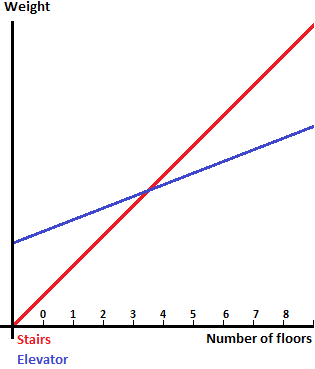
\includegraphics[width=0.5\textwidth]{stairsVSelevators.png}
    \label{fig:labeled_stairsVSelevators}
  \end{figure}